\documentclass[12pt, a4paper]{article}

% ===== 中文支持 =====
\usepackage[UTF8, zihao=-4]{ctex}

% ===== 页边距 =====
\usepackage[top=2.5cm, bottom=2.5cm, left=2.8cm, right=2.8cm]{geometry}

% ===== 字体 =====
\usepackage{fontspec}
\setmainfont{Times New Roman}

% ===== 行距 =====
\usepackage{setspace}
\setstretch{1.5}
\setlength{\parskip}{0pt}

% ===== 插图 =====
\usepackage{graphicx}
\usepackage{float}
\graphicspath{{./images/}{./实验图片/}}

% ===== 表格 =====
\usepackage{booktabs}
\usepackage{array}
\usepackage{multirow}

% ===== 数学公式 =====
\usepackage{amsmath, amssymb}

% ===== 图表编号（章-序号格式） =====
\usepackage{chngcntr}
\renewcommand{\thefigure}{\arabic{section}-\arabic{figure}}
\renewcommand{\thetable}{\arabic{section}-\arabic{table}}
\counterwithin{figure}{section}
\counterwithin{table}{section}

% ===== 图表标题 =====
\usepackage{caption}
\captionsetup{font=small, labelsep=space, justification=centering,
              aboveskip=6pt, belowskip=12pt}
\captionsetup[table]{aboveskip=12pt, belowskip=6pt, position=above}

% ===== 页眉页脚 =====
\usepackage{fancyhdr}
\setlength{\headheight}{15pt}
\pagestyle{fancy}
\fancyhf{}
\fancyhead[C]{\small 光学系统基点的测量\ 实验报告}
\fancyfoot[C]{\small\thepage}

% ===== 目录超链接 =====
\usepackage[colorlinks=true, linkcolor=black, citecolor=black, urlcolor=blue,
            bookmarks=true, bookmarksnumbered=true]{hyperref}

% ===== 章节标题格式（titlesec） =====
\usepackage{titlesec}
\titleformat{\section}[block]
  {\centering\heiti\zihao{4}}{\thesection}{1em}{}
\titlespacing*{\section}{0pt}{24pt}{18pt}
\titleformat{\subsection}[hang]
  {\heiti\zihao{-4}}{\thesubsection}{1em}{}
\titlespacing*{\subsection}{0pt}{18pt}{6pt}

\begin{document}

% ===== 封面 =====
\begin{titlepage}
  \centering
  \vspace*{3cm}
  {\heiti\zihao{2} 实验报告}\\[1cm]
  {\heiti\zihao{3} 光学系统基点的测量}\\[2.5cm]
  \begin{tabular}{ll}
    姓\quad 名： & 叶哲昊 \\[0.6cm]
    学\quad 号： & 24012561 \\[0.6cm]
    班\quad 级： & 24级光电二班 \\[0.6cm]
    实验日期：   & 2026.4.3 \\
  \end{tabular}
  \vfill
\end{titlepage}

\tableofcontents
\newpage
\setcounter{page}{1}

\section{实验目的}

\begin{enumerate}
  \item 了解共轴理想光学系统基点（主点/节点、焦点）的一般概念及特性；
  \item 掌握利用辅助透镜平行光法测定透镜组焦距 $f'$ 的实验方法；
  \item 学会由测定的焦点位置和焦距确定光学系统主点（节点）的空间位置；
  \item 将实验测量结果与理论值比较，分析误差产生的原因。
\end{enumerate}

\section{实验原理}

\subsection{主面和主点}

若将物体垂直于系统光轴放置在物方主点 $H$ 处，则必成一个与物体等大、正立的像于像方主点
$H'$ 处，即主点是横向放大率 $\beta = +1$ 的一对共轭点。过主点垂直于光轴的平面分别称为
物方主面（$MH$）和像方主面（$M'H'$），如图~\ref{fig:lens_diagram}~所示。

\begin{figure}[H]
  \centering
  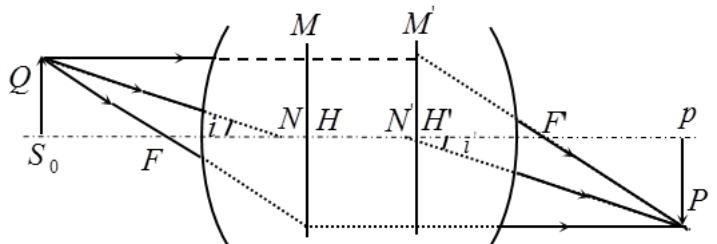
\includegraphics[width=0.68\textwidth]{b5ac16bc0cda2d7b04956dbd62f8ef256ef60c2fd3924555487b74e6211afc94.jpg}
  \caption{透镜组光路示意图}
  \label{fig:lens_diagram}
\end{figure}

\subsection{节点和节面}

节点是角放大率 $\gamma = +1$ 的一对共轭点。入射光线（或其延长线）过物方节点 $N$ 时，出射
光线（或其延长线）必过像方节点 $N'$，且两者方向平行。当光学系统两侧媒质相同（如空气）时，
节点与主点重合，即 $N \equiv H$，$N' \equiv H'$。

\subsection{焦点和焦面}

平行于系统主轴的平行光束经系统折射后与主轴的交点 $F'$ 称为像方焦点；像方主点 $H'$ 到像方
焦点 $F'$ 的距离称为像方焦距 $f'$。类似地，亦有物方焦点 $F$、物方焦距 $f$，在空气介质中
$f = -f'$。

\subsection{测量原理}

本实验以两薄透镜的组合系统为例。设 $L$ 为已知焦距 $f_0$ 的辅助凸透镜，L.S.\ 为待测透镜组，
其节点（主点）为 $N$、$N'$，像方焦点为 $F'$。将物 $AB$（高度 $h_1$）置于辅助透镜的前焦面
处，则出射为平行光，经 L.S.\ 后聚焦于后焦面，成像 $A'B'$（高度 $h_2$），见图~\ref{fig:measure_scheme}。

\begin{figure}[H]
  \centering
  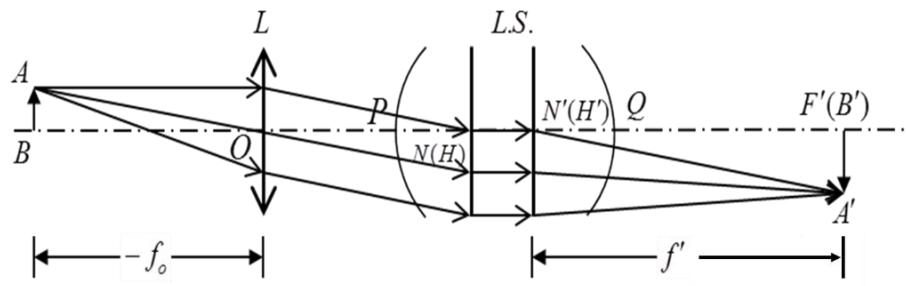
\includegraphics[width=0.70\textwidth]{a9cf378a00303dd6fa9399c9153d540332ea5d60294ac72a1a2053a4ee7e0e38.jpg}
  \caption{测量基点示意图}
  \label{fig:measure_scheme}
\end{figure}

由相似三角形 $\triangle AOB \sim \triangle A'N'B'$，得：

\begin{equation}
  \frac{AB}{-f_0} = \frac{A'B'}{f'}
  \label{eq:similar}
\end{equation}

取绝对值，像方焦距公式为：

\begin{equation}
  f' = f_0 \cdot \frac{h_2}{h_1}
  \label{eq:focal}
\end{equation}

式中 $h_1$、$h_2$ 均取正值（大小）。像 $A'B'$ 的位置即为像方焦点 $F'$，由 $F'$ 逆光方向
量取距离 $f'$ 即得像方主点（节点）$H'$（$N'$）。将透镜组旋转 $180^\circ$ 重复上述步骤，可
确定物方焦点 $F$ 和物方主点（节点）$H$（$N$）。

\subsection{理论焦距计算公式}

两薄透镜（焦距分别为 $f_1'$、$f_2'$，间距为 $d$）组合系统的像方焦距理论值为：

\begin{equation}
  f' = \frac{f_1' \cdot f_2'}{f_1' + f_2' - d}
  \label{eq:theory}
\end{equation}

本实验中固定透镜 $f_1' = 200\ \mathrm{mm}$，可动透镜 $f_2' = 350\ \mathrm{mm}$，间距
$d$ 可取 70、90、110\,mm。

\section{实验仪器}

本实验使用以下光学仪器：

\begin{enumerate}
  \item \textbf{"F"形 LED 光源}：作为发光物（目标板），"F"形标记用于成像观测，
        物高 $h_1 = 32.5\ \mathrm{mm}$（固定值）；
  \item \textbf{辅助透镜}：$\phi = 50\ \mathrm{mm}$，共两种焦距可选（75\,mm 或
        150\,mm），本次实验选用 $f_0 = 150\ \mathrm{mm}$，使目标板位于其前焦面
        以产生平行出射光；
  \item \textbf{节点镜头（待测透镜组）}：由两片透镜组成——固定透镜
        $\phi = 40\ \mathrm{mm}$、$f_1' = 200\ \mathrm{mm}$；可动透镜
        $\phi = 40\ \mathrm{mm}$、$f_2' = 350\ \mathrm{mm}$；两镜片间距可在
        $60\sim110\ \mathrm{mm}$ 范围内调节；
  \item \textbf{带刻度白屏（像屏）}：用于接收成像并测量像高 $h_2$；
  \item \textbf{光具座及导轨}：用于固定各光学元件并保证共轴对准；
  \item \textbf{毫米刻度尺}：用于测量物高、像高及各元件位置。
\end{enumerate}

实验装置全貌如图~\ref{fig:apparatus}~所示。

\begin{figure}[H]
  \centering
  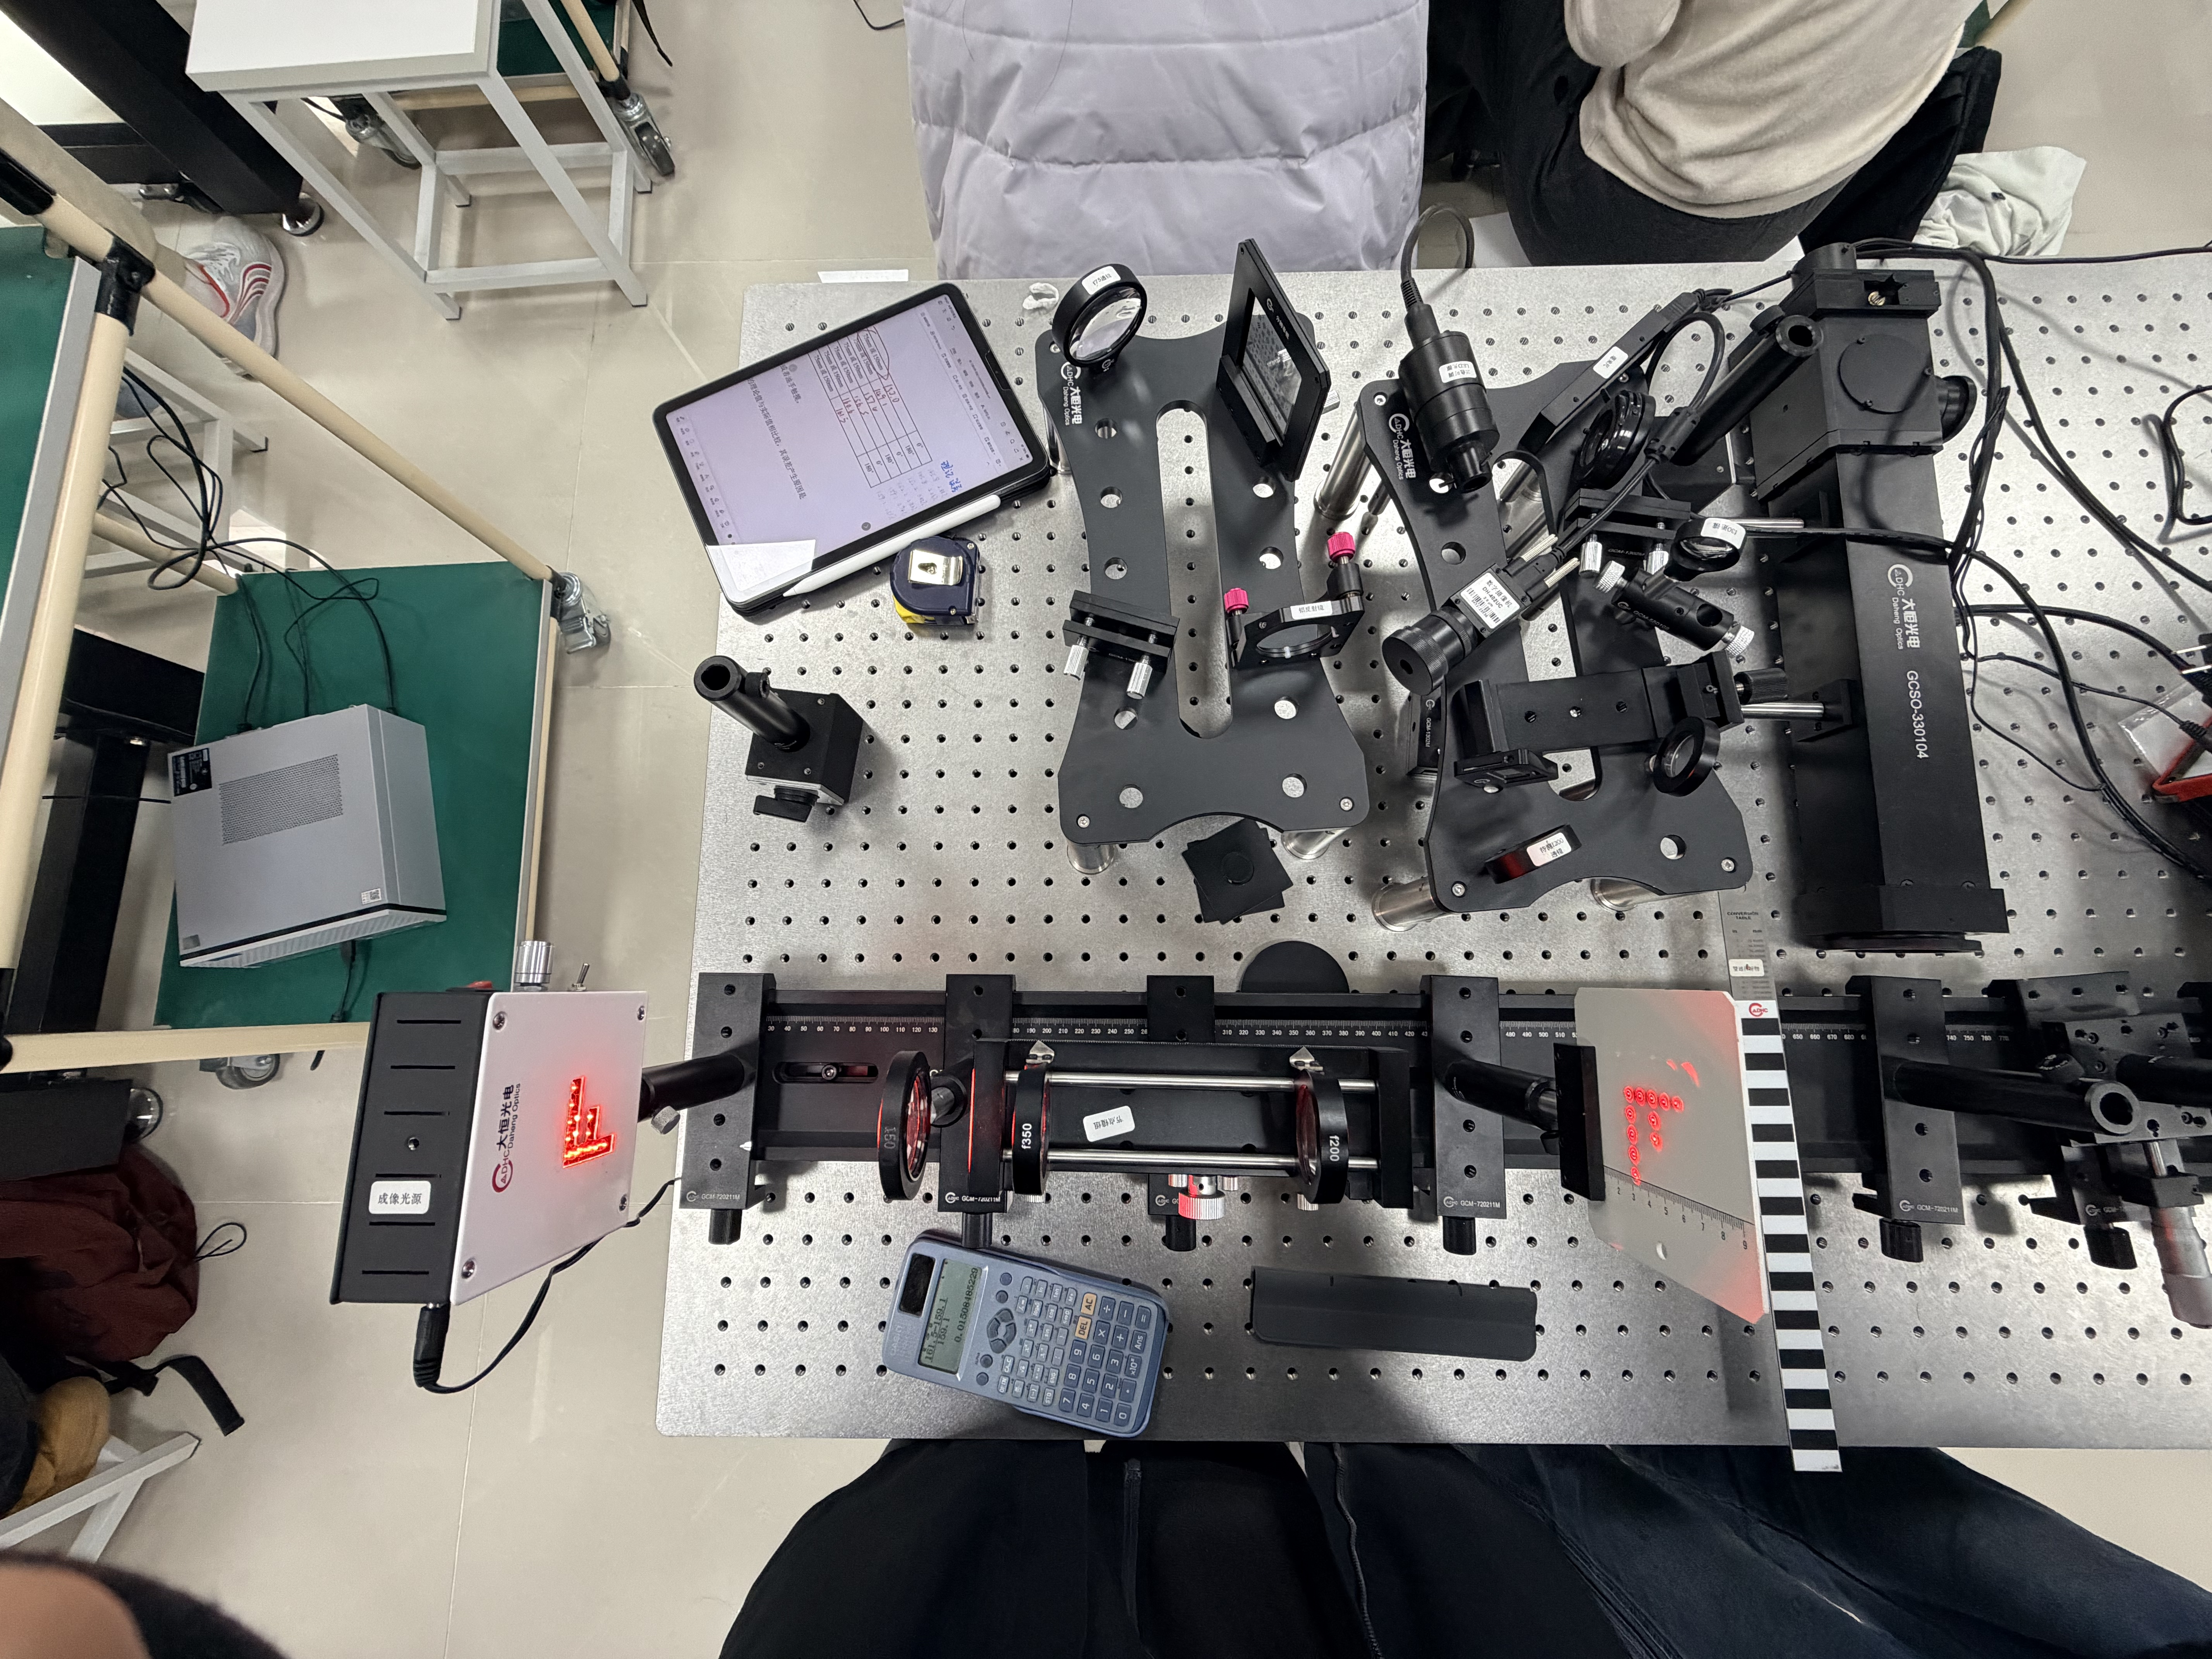
\includegraphics[width=0.80\textwidth]{实验装置全貌.jpg}
  \caption{实验装置全貌}
  \label{fig:apparatus}
\end{figure}

\section{实验步骤}

光路搭建示意如图~\ref{fig:setup_diagram}~所示，自左向右依次为光源、辅助透镜、节点镜头、
白屏。

\begin{figure}[H]
  \centering
  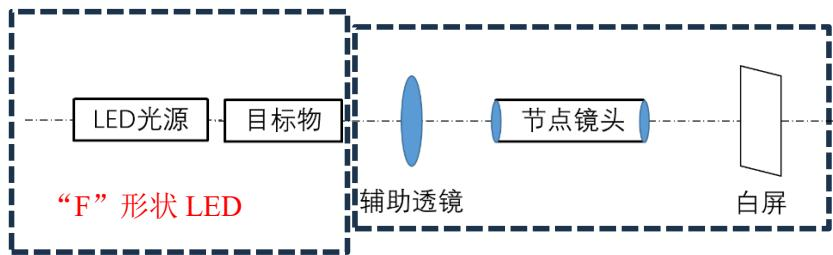
\includegraphics[width=0.78\textwidth]{0978bd91a0848c7d376d7c4dab760a2a7d5abf35aeb50ca1a10dc7b74386d047.jpg}
  \caption{透镜系统基点测量光路示意图}
  \label{fig:setup_diagram}
\end{figure}

\begin{enumerate}
  \item \textbf{安装光源与辅助透镜}：将"F"形 LED 光源置于光具座一端，在其后安装辅助凸
        透镜（$f_0 = 150\ \mathrm{mm}$），调整两者间距为 $150\ \mathrm{mm}$，即使目标板
        位于辅助透镜的前焦面，令出射光束近似为平行光。

  \item \textbf{安装节点镜头（$0^\circ$ 方向）}：将两薄透镜间距调至第一组实验值
        $d = 70\ \mathrm{mm}$，放置于辅助透镜后方并调整共轴，使光束入射到透镜中心。

  \item \textbf{找像、确定像方焦点 $F'$}：在节点镜头后放置白屏，沿光轴方向前后移动白屏
        直至观察到清晰的倒"F"像，此时白屏所在位置即为像方焦点 $F'$。

  \item \textbf{测量像高并记录数据}：用白屏刻度尺测量清晰像的高度 $h_2$（取绝对值），将
        $L$、$h_1$、$h_2$、$f_0$ 等数据填入表~\ref{tab:data}，备注栏标记为 $0^\circ$。

  \item \textbf{旋转 $180^\circ$，测物方焦点 $F$}：将节点镜头旋转 $180^\circ$，重复步骤
        3、4，确定物方焦点位置并记录对应 $h_2$，备注栏标记为 $180^\circ$。

  \item \textbf{改变间距，重复测量}：依次将间距改为 $d = 90\ \mathrm{mm}$ 和
        $d = 110\ \mathrm{mm}$，在 $0^\circ$ 和 $180^\circ$ 两方向各完成一次，共 6 组
        测量，结果填入表~\ref{tab:data}。

  \item \textbf{确定主点（节点）位置}：由 $F'$ 沿逆光方向量取距离 $f'$，即得像方主点
        $H'$（节点 $N'$）的位置；物方主点 $H$（节点 $N$）的位置由 $F$ 沿光行进方向量取
        $|f|$ 确定。
\end{enumerate}

\section{实验数据与处理}

\subsection{实验数据记录与焦距计算}

实验中辅助透镜焦距 $f_0 = 150\ \mathrm{mm}$，目标板物高 $h_1 = 32.5\ \mathrm{mm}$（固定）。
由式~(\ref{eq:focal}) 计算各组实验的焦距测量值，并与式~(\ref{eq:theory}) 所得理论值对比，
结果列于表~\ref{tab:data}。

\begin{table}[H]
  \centering
  \caption{节点镜头焦距记录与计算表（$f_0 = 150\ \mathrm{mm}$，$h_1 = 32.5\ \mathrm{mm}$）}
  \label{tab:data}
  \begin{tabular}{ccccccc}
    \toprule
    $L$/mm & $h_1$/mm & $h_2$/mm &
    $f'_{\mathrm{exp}}$/mm & $f'_{\mathrm{th}}$/mm & 相对误差 & 备注 \\
    \midrule
    70  & 32.5 & 32.5 & 150.0 & 145.8 & 2.88\% & $0^\circ$   \\
    70  & 32.5 & 32.3 & 149.1 & 145.8 & 2.26\% & $180^\circ$ \\
    90  & 32.5 & 34.1 & 157.4 & 152.2 & 3.42\% & $0^\circ$   \\
    90  & 32.5 & 33.9 & 156.5 & 152.2 & 2.83\% & $180^\circ$ \\
    110 & 32.5 & 34.8 & 160.6 & 159.1 & 0.94\% & $0^\circ$   \\
    110 & 32.5 & 35.0 & 161.5 & 159.1 & 1.51\% & $180^\circ$ \\
    \bottomrule
  \end{tabular}
\end{table}

\subsection{计算示例}

以 $L = 70\ \mathrm{mm}$、$0^\circ$ 方向为例，由式~(\ref{eq:focal}) 得：

\begin{equation}
  f' = f_0 \cdot \frac{h_2}{h_1} = 150 \times \frac{32.5}{32.5} = 150.0\ \mathrm{mm}
\end{equation}

相对误差为：

\begin{equation}
  \delta = \frac{|f'_{\mathrm{exp}} - f'_{\mathrm{th}}|}{f'_{\mathrm{th}}}
         = \frac{|150.0 - 145.8|}{145.8} \approx 2.88\%
\end{equation}

\subsection{理论焦距计算}

由式~(\ref{eq:theory})，$f_1' = 200\ \mathrm{mm}$，$f_2' = 350\ \mathrm{mm}$，各间距对应
理论焦距如下：

$d = 70\ \mathrm{mm}$：
\begin{equation}
  f'_{\mathrm{th}} = \frac{200 \times 350}{200 + 350 - 70}
                   = \frac{70000}{480} \approx 145.8\ \mathrm{mm}
\end{equation}

$d = 90\ \mathrm{mm}$：
\begin{equation}
  f'_{\mathrm{th}} = \frac{200 \times 350}{200 + 350 - 90}
                   = \frac{70000}{460} \approx 152.2\ \mathrm{mm}
\end{equation}

$d = 110\ \mathrm{mm}$：
\begin{equation}
  f'_{\mathrm{th}} = \frac{200 \times 350}{200 + 350 - 110}
                   = \frac{70000}{440} \approx 159.1\ \mathrm{mm}
\end{equation}

\section{实验结果与分析}

\subsection{焦距测量结果}

完成 6 组实验，三种镜片间距下的焦距测量值与理论值对比良好，所有相对误差均在
$3.5\%$ 以内（最大误差 $3.42\%$，最小误差 $0.94\%$）。随镜片间距 $d$ 增大，
系统焦距 $f'$ 单调增大，与式~(\ref{eq:theory}) 的理论预期一致：间距从
70\,mm 增至 110\,mm，实验平均焦距从约 149.6\,mm 升至约 161.1\,mm，
增幅约 11.5\,mm，理论增幅为 $159.1-145.8=13.3\ \mathrm{mm}$，趋势相符。

\subsection{主点（节点）位置的确定}

以 $d = 70\ \mathrm{mm}$ 为例（$0^\circ$ 方向），像屏清晰成像处即为像方焦点
$F'$，由 $F'$ 沿逆光方向量取 $f' = 150.0\ \mathrm{mm}$ 即得像方主点（节点）
$H'$（$N'$）的位置。旋转 $180^\circ$ 后类似地确定物方焦点 $F$ 和物方主点
（节点）$H$（$N'$）的位置。实验中白屏上观察到的清晰倒"F"像如图~\ref{fig:screen}~所示。

\begin{figure}[H]
  \centering
  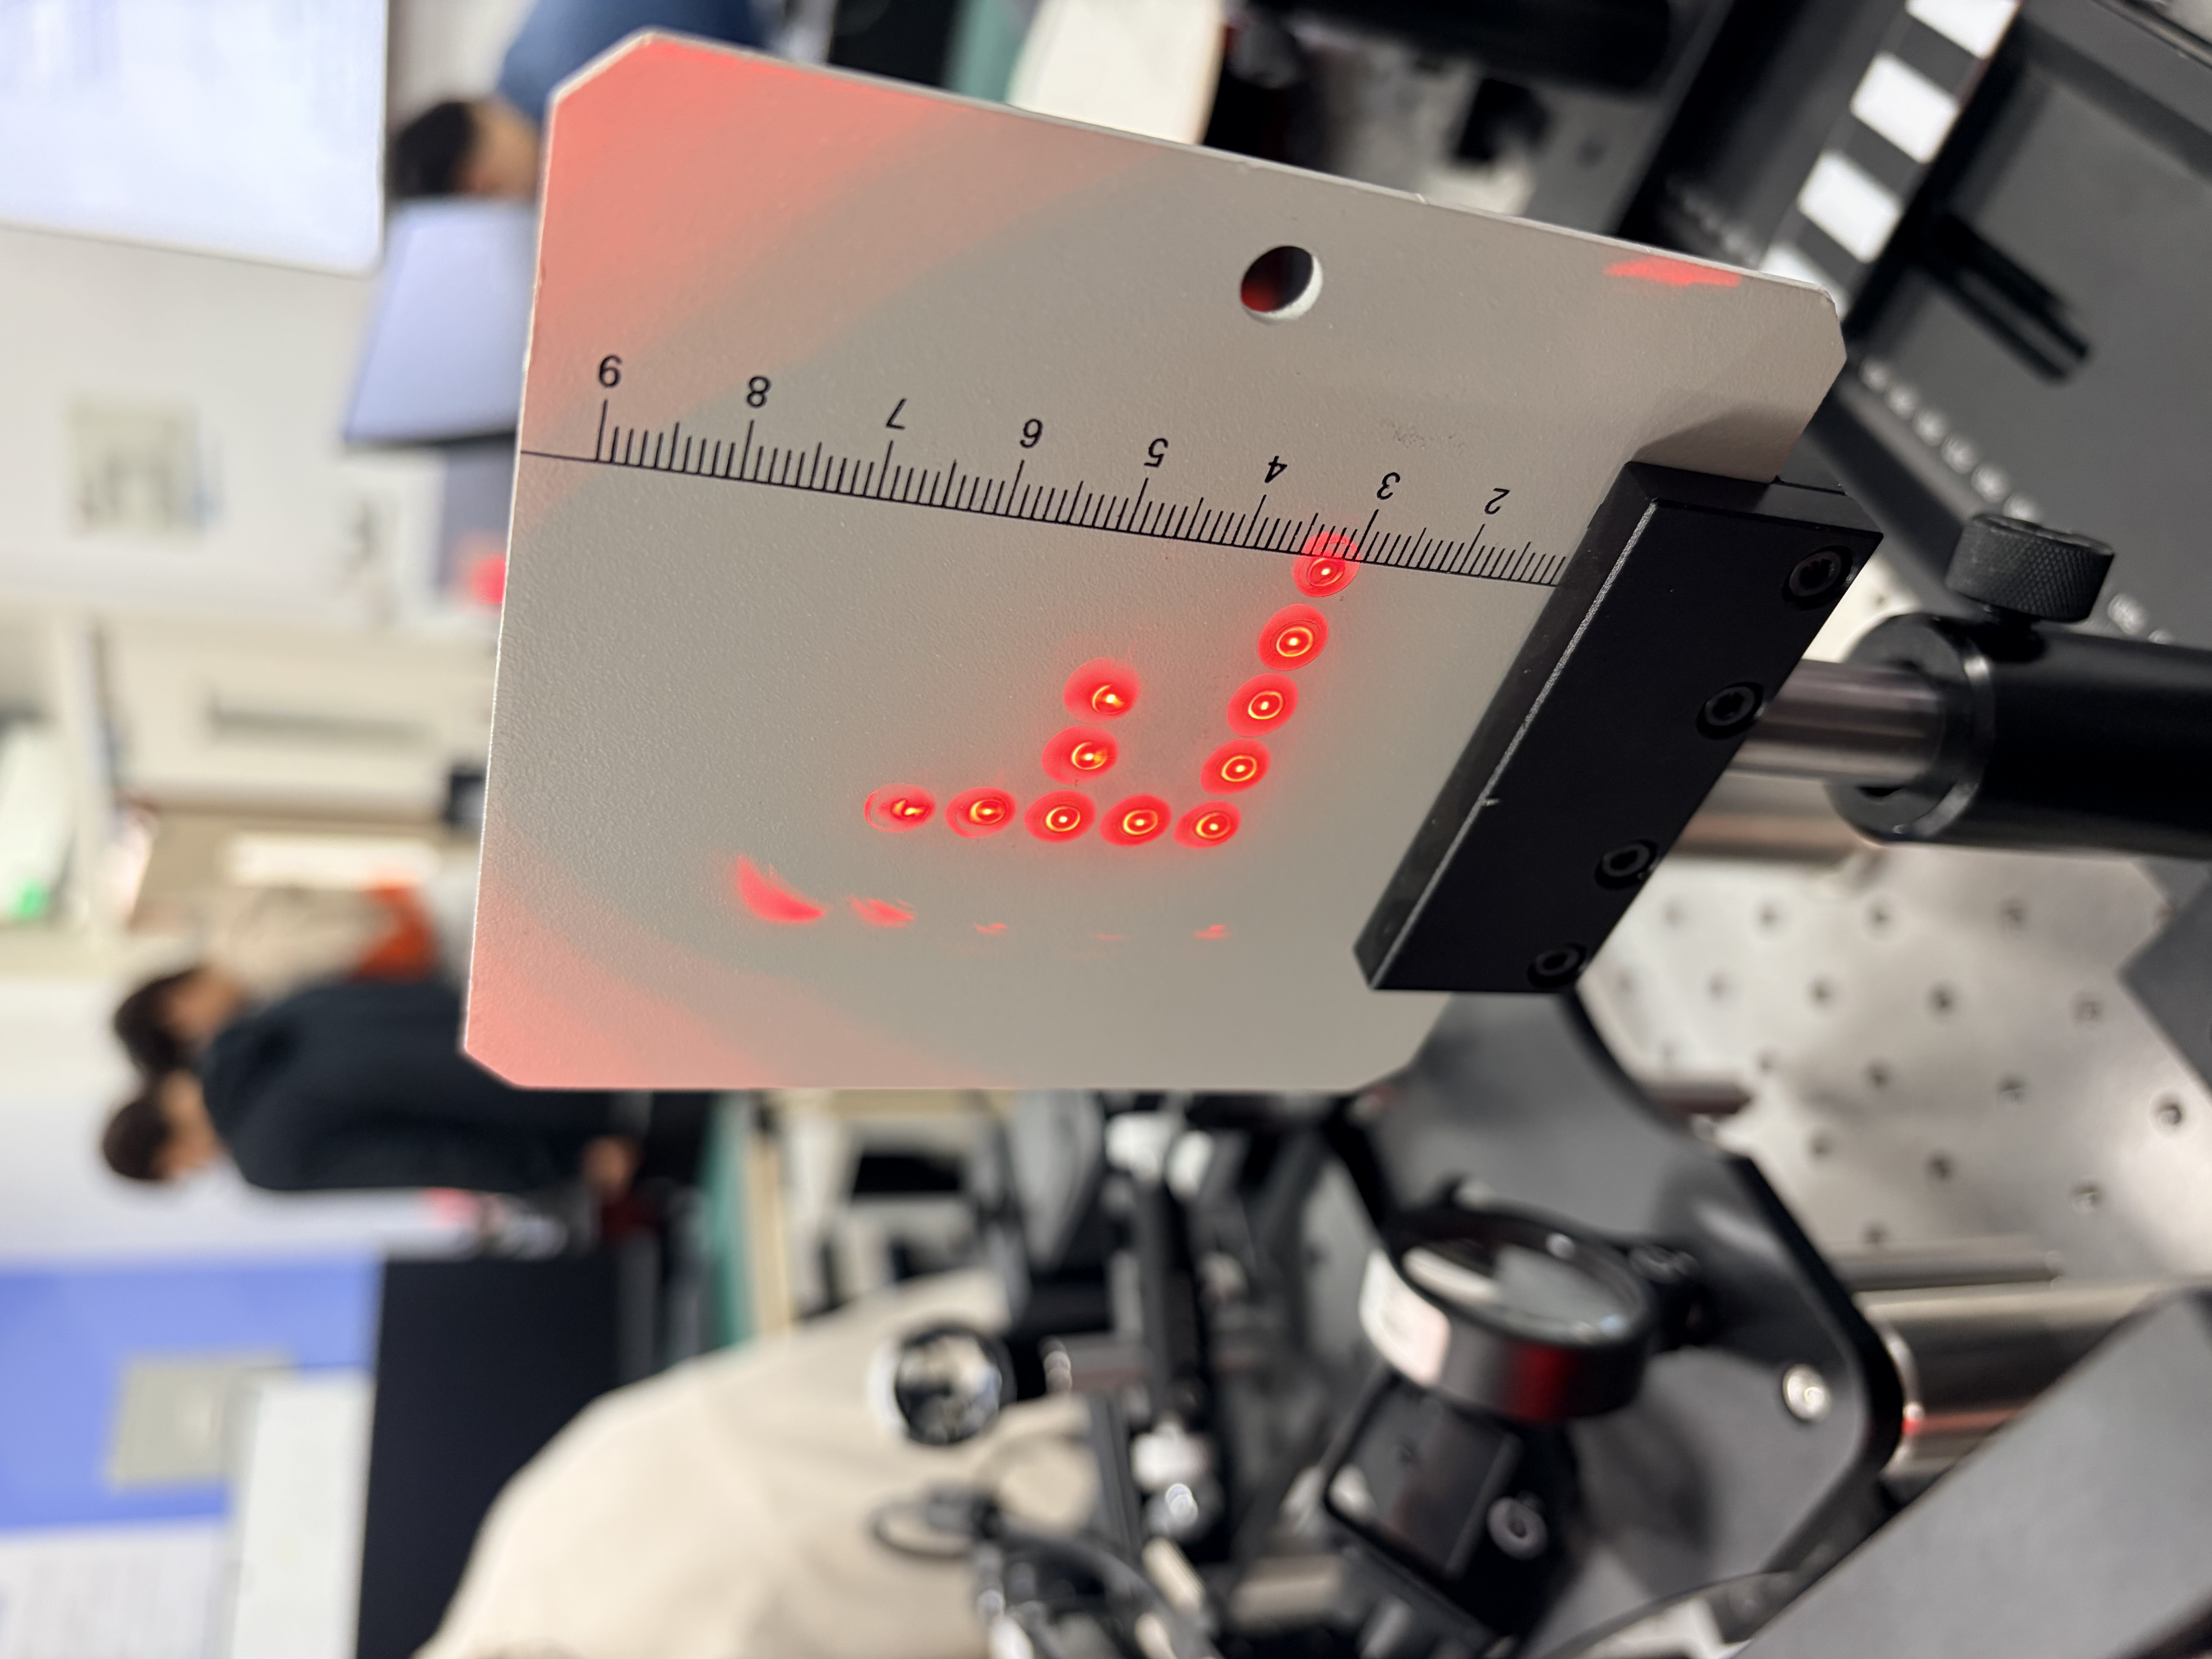
\includegraphics[width=0.50\textwidth]{光屏细节.jpg}
  \caption{白屏上清晰的倒"F"像（$d = 70\ \mathrm{mm}$，$0^\circ$ 方向）}
  \label{fig:screen}
\end{figure}

\subsection{$0^\circ$ 与 $180^\circ$ 结果对比}

同一间距下，$0^\circ$ 与 $180^\circ$ 测得的焦距（分别为前向像方焦距与物方焦距）
数值接近但不完全相同，反映了实际透镜组正反两侧焦距的微弱不对称，亦包含了两次独立
实验的随机误差，总体一致性较好。

\section{误差分析}

本实验的误差来源主要包括以下几个方面：

\begin{enumerate}
  \item \textbf{像高测量误差}：像高 $h_2$ 由白屏上的刻度尺目视读数，存在视差和主观判断
        误差，每次约有 $\pm 0.5\ \mathrm{mm}$ 的读数不确定度，是本实验最主要的误差来源。
        由误差传递公式，$f'$ 的相对不确定度约为 $|{\Delta h_2}/{h_2}|$。

  \item \textbf{调焦不准确}：白屏位置是否精确对应最清晰的成像存在主观判断偏差（焦深效应），
        导致像方焦点 $F'$ 定位存在偏差，从而影响 $f'$ 的测量精度和主点位置的确定。

  \item \textbf{光轴共轴误差}：各光学元件若未精确共轴（倾斜或横向偏移），会引入附加像差，
        使像质下降并影响像高读数。

  \item \textbf{薄透镜近似误差}：理论公式~(\ref{eq:theory}) 基于薄透镜模型，而实际透镜
        有一定厚度，主面位置与薄透镜几何中心存在偏差，引入系统性误差。

  \item \textbf{辅助透镜定位误差}：若目标板未精确位于辅助透镜前焦面处（间距偏离
        $f_0 = 150\ \mathrm{mm}$），则出射光非严格平行，使实际入射到待测系统的不再是理想
        平行光，造成测量偏差。

  \item \textbf{透镜间距读数误差}：镜片间距 $d$ 的读数若有偏差，由式~(\ref{eq:theory})
        可知会影响理论值计算，但此项对实验测量值无直接影响，仅影响误差评估的准确性。
\end{enumerate}

\section{实验结论}

本实验采用"辅助透镜平行光法"，成功测定了节点镜头（两薄透镜组合）在三种镜片间距下的像方
和物方焦距，并由焦点位置结合焦距确定了主点（节点）的位置。主要结论如下：

\begin{enumerate}
  \item 实验测量焦距值与理论公式~(\ref{eq:theory}) 计算结果的相对误差均在 $3.5\%$ 以内，
        验证了两薄透镜组合系统焦距公式的正确性。

  \item 在空气介质中，光学系统的节点与主点完全重合。通过确定焦点位置并量取焦距，即可同时
        确定节点和主点的位置，实验方法简便有效。

  \item 增大镜片间距 $d$ 可使系统焦距 $f'$ 增大，实验结果定性、定量均与理论预期相符，为
        光学系统设计中通过调节间距改变焦距提供了实验依据。

  \item 实验误差主要来自像高目视读数的随机误差和调焦判断的主观不确定性。为提高精度，宜
        多次测量取平均、仔细调节共轴，并注意辅助透镜的精确定位。
\end{enumerate}

\end{document}
